%%
% This is an Overleaf template for presentations
% using the TUM Corporate Desing https://www.tum.de/cd
%
% For further details on how to use the template, take a look at our
% GitLab repository and browse through our test documents
% https://gitlab.lrz.de/latex4ei/tum-templates.
%
% The tumbeamer class is based on the beamer class.
% If you need further customization please consult the beamer class guide
% https://ctan.org/pkg/beamer.
% Additional class options are passed down to the base class.
%
% If you encounter any bugs or undesired behaviour, please raise an issue
% in our GitLab repository
% https://gitlab.lrz.de/latex4ei/tum-templates/issues
% and provide a description and minimal working example of your problem.
%%

\documentclass[
  german,            % define the document language (english, german)
  aspectratio=169,    % define the aspect ratio (169, 43)
  % handout=2on1,       % create handout with multiple slides (2on1, 4on1)
  % partpage=false,     % insert page at beginning of parts (true, false)
  % sectionpage=true,   % insert page at beginning of sections (true, false)
]{tumbeamer}


% load additional packages
\usepackage{booktabs}
\usepackage{graphicx}
\usepackage{tikz}
\usepackage{url}
\usepackage{pgfplots}
\usepackage{hyperref}
\usepackage{pmboxdraw}
\usepackage{float}
\usepackage{babel}[ngerman]
\usepackage{csquotes}[autostyle]
\usepackage[useregional]{datetime2}
\usepackage{listings}
\usepackage{xurl}
\usepackage{enumerate}
\usepackage{circuitikz}
\usepackage{csquotes}
\usepackage{tikz-timing}

%\usepackage{minted}
%\usemintedstyle{borland}
\usetikzlibrary{patterns}
\pgfplotsset{compat=1.18}

% tikz
\usetikzlibrary{overlay-beamer-styles}
\usetikzlibrary{arrows,backgrounds,positioning,shapes,,patterns,patterns.meta,matrix,arrows,shapes.geometric}
\usetikzlibrary{matrix}
% requires circuitikz >= 1.1.0
% for distros with older distributions, install TeX Live manually
% instead of using your package manager
% see: https://tug.org/texlive/quickinstall.html
\ctikzset{logic ports=european}

% minted

\lstset {
    frame=single,
    tabsize=4,
    breaklines=true,
    xleftmargin=5pt,
    xrightmargin=5pt,
    basicstyle=\ttfamily\footnotesize,
    %language=[RISC-V]Assembler,
}

\hypersetup { 
  colorlinks=true,
  urlcolor=blue,
  filecolor=black,
  linkcolor=black
}

% tikz  
\usetikzlibrary{fit}

% image path
\graphicspath{ {../resources/} }

% presentation metadata
\title{Übung 08: RISC-V Single-Cycle Prozessor}

\subtitle{Einführung in die Rechnerarchitektur}

\author{\theAuthorName}

\institute{\theGroupName\\\theSchoolName\\\theUniversityName}
\date{9. -- \DTMdisplaydate{2024}{12}{15}{-1}}

\footline{\insertauthor~|~\insertshorttitle~|~\insertshortdate}


% macro to configure the style of the presentation
\TUMbeamersetup{
  title page = TUM tower,         % style of the title page
  part page = TUM toc,            % style of part pages
  section page = TUM toc,         % style of section pages
  content page = TUM more space,  % style of normal content pages
  tower scale = 1.0,              % scaling factor of TUM tower (if used)
  headline = TUM threeliner,      % which variation of headline to use
  footline = TUM default,         % which variation of footline to use
  % configure on which pages headlines and footlines should be printed
  headline on = {title page},
  footline on = {every page, title page=false},
}


% available frame styles for title page, part page, and section page:
% TUM default, TUM tower, TUM centered,
% TUM blue default, TUM blue tower, TUM blue centered,
% TUM shaded default, TUM shaded tower, TUM shaded centered,
% TUM flags
%
% additional frame styles for part page and section page:
% TUM toc
%
% available frame styles for content pages:
% TUM default, TUM more space
%
% available headline options:
% TUM empty, TUM oneliner, TUM twoliner, TUM threeliner, TUM logothreeliner
%
% available footline options:
% TUM empty, TUM default, TUM infoline

\begin{document}

\maketitle

\begin{frame}[c]{Mitschriften \& Infos}{}
  \begin{minipage}[t]{\textwidth}
    \begin{columns}[c]
      \begin{column}{0.8\textwidth}
        Montags: \href{\zulipMo}{\zulipMo}
      \end{column}
      \begin{column}{0.2\textwidth}
        \includegraphics[width=0.8\linewidth]{\zulipMoQrFilename}
      \end{column}
    \end{columns}
  \end{minipage}
  \rule{\textwidth}{0.4pt}
  \begin{minipage}[t]{\textwidth}
    \begin{columns}[c]
      \begin{column}{0.8\textwidth}
        Donnerstags: \href{\zulipDo}{\zulipDo}
      \end{column}
      \begin{column}{0.2\textwidth}
        \includegraphics[width=0.8\linewidth]{\zulipDoQrFilename}
      \end{column}
    \end{columns}
  \end{minipage}
  \ifdefined\myWebsite
  \rule{\textwidth}{0.4pt}
  \centering
  Website: \href{\myWebsite}{\myWebsite}
  \fi
\end{frame}

\begin{frame}[c]{}{}
  \begin{center}
    \LARGE  Keine Garantie für die Richtigkeit der Tutorfolien.

    \Large Bei Unklarheiten/Unstimmigkeiten haben VL/ZÜ-Folien recht!
  \end{center}
\end{frame}

\begin{frame}[c]{Inhaltsübersicht}{}
  \begin{columns}[c]
    \begin{column}{1\textwidth}
      \begin{itemize}
        \item Quiz
        \item Wiederholung
        \item Tutorblatt
        \begin{itemize}
          \item Lösungsvorschläge
          \item Fehlerhafte Kontrollsignale
          \item Erweiterung: BNE
          \item Kontrollsignalbelegung
        \end{itemize}
      \end{itemize}
    \end{column}
  \end{columns}
\end{frame}

\begin{frame}[c, fragile]{}{}
  \begin{center}
    \vspace{0.5cm}
    \begin{block}{Zitat der Woche}
      \vspace{0.5cm}
      \begin{quote}
        \enquote{So funktioniert die Welt am Ende auch. Man braucht halt seine Vollidioten für jedes Gebiet -- ich bin der Vollidiot für Informatik. Es gibt andere Vollidioten für Elektrotechnik. So halten wir die Welt zusammen.}
        \vspace{0.5cm}
        \flushright{\textbf{-- Prof. Dr. Robert Wille (Vollidiot für Informatik)}}
      \end{quote}
      \vspace{0.5cm}
    \end{block}
    \vspace{0.5cm}
    Quelle: \href{https://tum.live/w/ws24EidR/50024?t=3005}{Lecture: November 26. 2024 (tum.live)}
\end{center}
\end{frame}

\begin{frame}[c, fragile]{RISC-V Instruktionstypen}{}
	\begin{itemize}
		\item R-Typ: Register-Register-Operationen (bspw. \texttt{add}, \texttt{sub}, \texttt{sll})
		\item I-Typ: kleine Immediates (12 Bit) und Ladebefehle (bspw. \texttt{jalr}, \texttt{lw}, \texttt{ori})
		\item U-Typ: große Immediates (20 Bit) (bspw. \texttt{lui}, \texttt{auipc})
		\item S-Typ: Speicherbefehle (bspw. \texttt{sw}, \texttt{sh})
		\item B-Typ: Branches (bedingte Sprünge) (bspw. \texttt{beq}, \texttt{blt}, \texttt{bgtu})
		\item J-Typ: Jumps (unbedingte Sprüge) (\texttt{jal})
	\end{itemize}
\end{frame}

\begin{frame}[c, fragile]{Assemblierung zu Maschinensprache}{}
	\begin{columns}[c]
		\begin{column}{0.5\textwidth}
			\begin{itemize}
				\item RV32: Instruktionsgröße von 32 Bit (compressed instructions 16 Bit)
				\item Übersetzung in CISC-Architekturen aufwendiger (vgl. IA-32: 2552 Seiten Instruction Reference)
				\item Instruktionen selben Typs werden haben gleiches Instruktionslayout
				\item alle benötigten Tabellen sind in der Klausur gegeben
			\end{itemize}
		\end{column}
		\begin{column}{0.5\textwidth}
			\begin{center}
				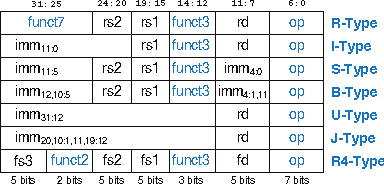
\includegraphics[width=\textwidth]{w08_risc_v_types.pdf}\\
			\end{center}
			\centering
			\tiny (Quelle: Vorlesungsmaterialien ERA)
		\end{column}
	\end{columns}
\end{frame}

\begin{frame}[c, fragile]{Assemblierung zu Maschinensprache: Beispiel}{}
	\begin{center}
		\large\texttt{xor t2, t1, t0}\\
		\scriptsize
		\begin{table}[]
			\begin{tabular}{|l|l|l|l|l|}
				\hline
				\rowcolor[HTML]{0078C3}
				{\color{white}\textbf{op}} & {\color{white}\textbf{funct3}} & {\color{white}\textbf{funct7}} & {\color{white}\textbf{Type}} & {\color{white}\textbf{Instruction}} \\ \hline
				0110011 (51)               & 100                            & 0000000                        & R                            & \texttt{xor rd, rs1, rs2}           \\ \hline
			\end{tabular}
		\end{table}

		
\includegraphics[width=0.59\textwidth]{w08_r_type.pdf}
	\end{center}

	\begin{enumerate}
		\item \texttt{xor} $\rightarrow$ R-Typ
		\item \texttt{t0} $\rightarrow$ \texttt{x5} (rs2), \texttt{t1} $\rightarrow$ \texttt{x6} (rs1), \texttt{t2} $\rightarrow$ \texttt{x7} (rd)
		\item funct7, funct3, op aus Tabelle ablesen
	\end{enumerate}
	\begin{center}
		\Large
		$(0000000\;00101\;00110\;100\;00111\;0110011)_2 = \textrm{0x005343B3}$
	\end{center}

\end{frame}


\begin{frame}[c]{RISC-V Single-Cycle-Prozessor}{}
	\begin{center}
		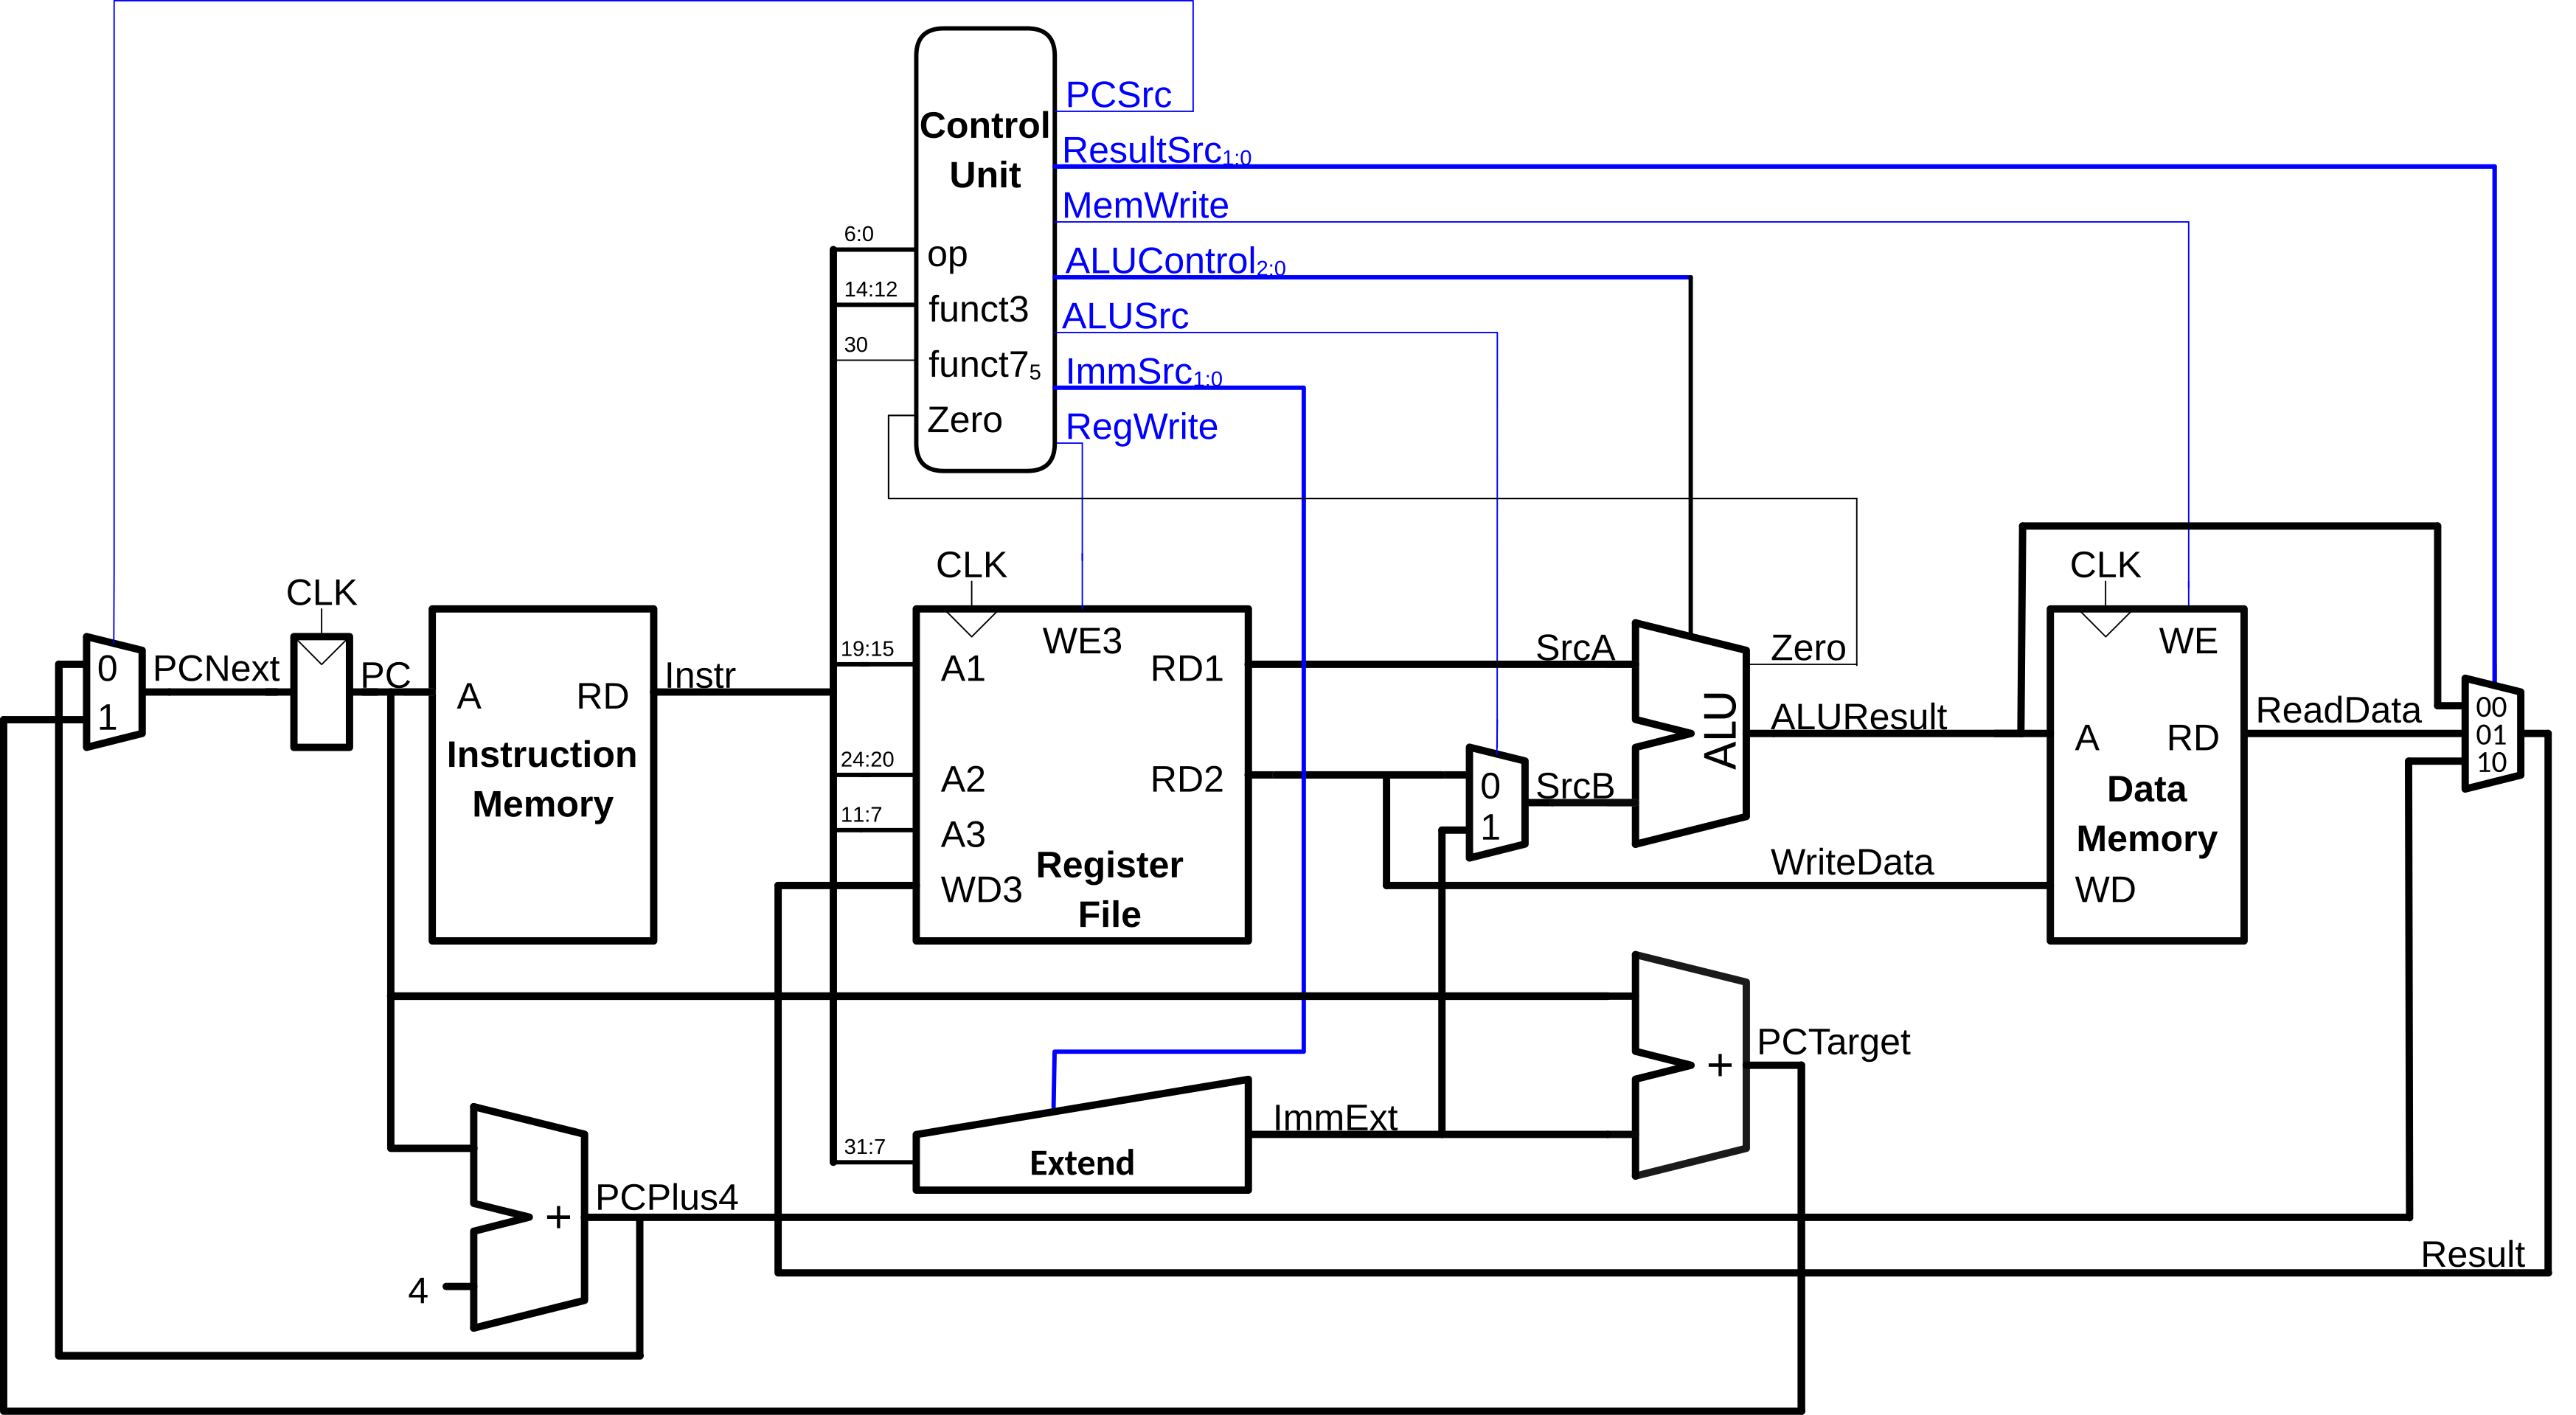
\includegraphics[width=0.8\textwidth]{w08_single_cycle.png}
	\end{center}
	\centering
	\tiny (Quelle: Vorlesungsmaterialien ERA)
\end{frame}

\begin{frame}[c, fragile]{}{}
	\begin{center}
		\LARGE Fragen?
	\end{center}
\end{frame}

\begin{frame}[c]{}{} 
  \begin{center}
    \LARGE Fragen?
  \end{center}
  \vspace{0.5cm}
  \begin{center}
    \LARGE Bis zum nächsten Mal ;) \\
  \end{center}
  \vspace{1.0cm}
  \begin{center}
    \small Folien inspiriert von Niklas Ladurner und Prof. Dr. Robert Wille
  \end{center}
\end{frame}

\end{document}